\chapter{Introduction}
The advantage of quantum computing lies in the possibility of parallel computing. The use of quantum communication has been in key distribution.

\section{The power of parallel computing}
Maze problems are hard because there are too many paths to explore from the entrance to the exit. If changing the question of the problems from pinpointing the actual paths to finding the number of good paths, although seemingly dumb down, the challenge is as hard as the original. One still needs to explore all the possible paths to reach the conclusion.

\begin{figure}[ht]
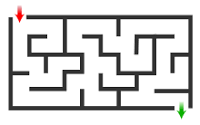
\includegraphics[width=6cm]{pic/maze.png}
\caption{Maze}
\label{Maze}
\end{figure}

Computer scientists have long known parallel computing is the way to speed up solutions to such problems. But how to realize parallel computing needs the help of physicists. Indeed, a physicist would suggest the following experiment to attack the problem: run water into the entrance and observe what's coming out of the exit. If we see water out of the exit, we know the maze has at least one good path. Of course, this is not the ultimate answer. But at least it shows the power of using water for parallel exploration.

We can obtain more information if we explore the water experiment further: put one big drop of water into the entrance and observe how many drops of water coming out. If three drops coming out of the exit, we can conclude that the maze has at least three good paths. We can also conclude the relative lengths of the paths by measuring the time delays of the three drops assuming water runs through all the paths at the same speed. In another word, the timing of the exiting water drops carries the length information of the paths.

One problem left is whether we can determine for sure that each of the three drops corresponds to one or more paths. For this, water is not a good medium because a water drop can always be divided up into smaller drops. Having a smallest drop, which cannot be further divided, must be included in the characteristics of a perfect medium for our parallel computing experiments:
\begin{itemize}
    \item it must be able to spread and to explore all possible solutions
    \item it must have one or more parameters, such as the time delay of a water drop, that can carry information
    \item it can be broken up into one or more smallest drops.
\end{itemize}
Many media possess the first two characteristics. But only quantum waves possess all three.

\section{The quantum power}
Quantum physics tells us that all waves have their smallest drops -- the quanta, which cannot be divided further. This is the so-called particle nature of waves. Quantum physics also says that all matters including electrons and protons are waves. Physicists refer the two concepts as the particle and wave dual-natures of matters. They are the essence of quantum physics. Their truthfulness have been proven by millions of experiments and more importantly by the advance of technologies including semiconductor and superconductor technologies.

The first hint of quantum power for parallel computing came by the proposal of Deutsch's algorithm\cite{1985Deutsch}. Shor's algorithm, published in 1997, is an extension of Deutsch's algorithm in scale as we will explain. But it shocks the world by its potential power of factoring large numbers and, as a consequence, breaking modern encryption technologies.

The hint of applying quantum physics to secure communication came in 1984 by the publication of the BB84 protocol\cite{BB84}. The fact that the smallest drop of a quantum wave cannot be divided prevents it from being partially tapped for eavesdropping. In our daily life, we are already used to the parallel capability of Wi-Fi waves, which allows communication with multiple devices simultaneously. Let's assume the antennae of our Wi-Fi box at home sends out 3 quanta of the wave at a time to limit the communication to precisely 3 devices. If the third device fails to receive its quantum of wave, it knows that someone has tapped it.

\subsection{The particle nature}
To most people, particles have the image of point-like things with negligible sizes but observable locations. This image is wrong and leads to all the misunderstandings about quantum physics. The particle nature really refers to the fact that all matters have the smallest drops when measured by their energy, mass or charge. For electrons and protons, measuring their mass or charge shows the smallest drops. For lights or electromagnetic waves, measuring their energy shows the smallest drops, and each drop is called a photon. We shall use the term quantum instead of particle when referring to photons and electrons in general.

We must remember that the only parameters that describe the particle or quantum nature of waves are their energy, mass and charge. Sizes or locations must not be used to describe quanta. If we do, paradoxes such as Einstein–Podolsky–Rosen (EPR) paradox \cite{EPR} are unavoidable.

The quantum nature of waves gives us the precision needed for parallel computing. But on the other hand, a quantum of a wave can only be measured once. A measurement requires energy to be extracted from the wave to the measurement device. And the phase, the conjugate variable of energy, becomes uncertain, and any information carried by it is lost forever.

\subsection{The wave nature}
When talking about waves, we often visualize ripples in a lake or the surges in oceans and seas. We observe water being pushed up and then pulled down by gravity. When we shake one end of a string as show in Fig. \ref{String}, we also see the vibration of each section of the string and the propagation of the vibration. Our perception of a wave includes something vibrating and the vibration propagating. But can we consider the vibration of a guitar string a wave? Indeed, we can. The reason we don't perceive the vibration propagating is because it gets reflected back by the two fixed ends of the string. Therefore, propagation or spatial spread remains a defining characteristic of waves, even if their propagation or spread is constrained.

Quantum computing and communication use only electromagnetic waves and electron waves, whose vibrations are not visible as a wave of a string. But they behave similarly.

\begin{figure}[ht]
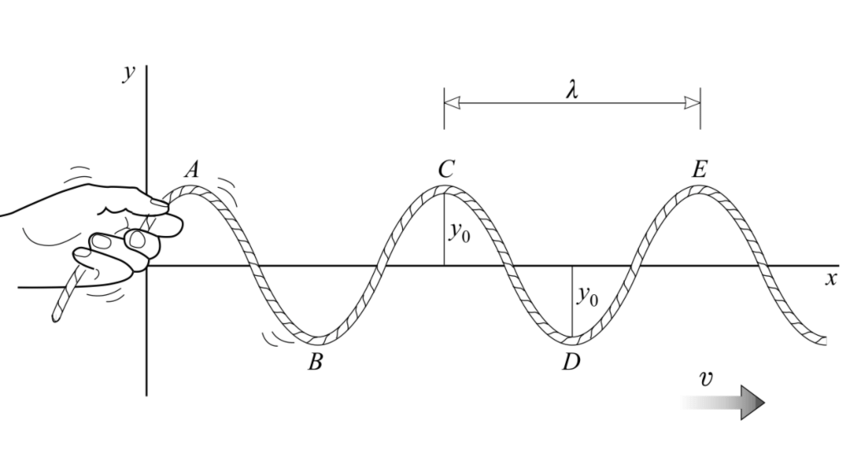
\includegraphics[width=6cm]{pic/wave-in-a-string.png}
\caption{Wave arisen from shaking or vibrating one end of a string.}
\label{String}
\end{figure}

\subsubsection{Types of waves by propagating characteristics}
Radio-frequency (RF) electromagnetic waves are used for mobile communications including Wi-Fi. They can spread to everywhere if not being blocked or confined by reflective matters. Light waves -- electromagnetic waves with wavelength ranging from sub-micron to a few microns -- are used for optical communications. They can be channeled by optical waveguides such as optical fibers to explore different paths. They are confined in two dimensions -- the lateral dimensions -- but propagate in the dimension along the axes of the waveguides or fibers. Communication, quantum or not, must use propagating waves, of course. With difficulties, propagating waves may also be used in quantum computing.

A wave does not have definite size or location unless it is confined. If an electromagnetic wave is confined in three dimensions, such as in a microwave oven, the wave cannot propagate anywhere other than being reflected back and forth. Only standing waves of specific frequencies can exist within such a confinement. The allowed frequencies are discrete. Standing waves are good for storing information. Superconductor qubits are built by standing waves of electrons as we discuss in the appendix. Standing waves may be best visualized and understood by the vibrations of a guitar string. When a string is plucked, the propagation of the vibrations are stopped and reflected by the two fixed ends. Only the waves whose phases coincide after a complete round trip of reflection survive while the other waves cancel each other and die off.

Another type of waves, which we may call trapped waves, are not confined with clear boundaries but are trapped by forces extending to infinity. Electrons in an atom are trapped waves by the electric force of the nucleus' positive charges. The waves extend to infinity but are concentrated within a nanometer around the nucleus. Trapped waves are also good for storing information. Trapped-ion qubits are built by trapped electron waves.

%\tdplotsetmaincoords{60}{120} % Set the viewpoint angles (adjust as needed)

%\begin{tikzpicture}%[tdplot_main_coords]
% Draw the outer surface of the tube
%\draw (0,0) ellipse (0.8cm and 2cm);
%\draw (5,0) ellipse (0.8cm and 2cm);

% Draw the inner surface of the tube (representing the hollow part)
%\draw (0,0) ellipse (0.5cm and 1.5cm);

% Connect the ends of the cylinders to form the tube
%\draw (0,-2) -- (5,-2);
%\draw (0,2) -- (5,2);
%\end{tikzpicture}

\subsubsection{Information representation by wave characteristics}
When we get our blood pressure measured in a doctor's office, the height of the mercury in a glass column represents the information of our blood pressure. The height of mercury in the column is what we actually measure and is what we use the height of a mercury in a cylinder to represent the information of our blood pressure. We see that physical characteristics, which can be measured in numbers, can be used to represent information. Information theory assumes all information can be presented as numbers. In turn, engineers and physicists use physical characteristics that can be measured in numbers to represent the information. In quantum computing and communication, information is represented by wave characteristics. When processing or transmitting certain information, it is first mapped to numbers before the numbers are mapped to some wave characteristics. The first step is called encoding, and the second step is modulation in the traditional communication terminology.
\begin{table}[]
\caption{Information represented by physical characteristics}
\label{information-characteristics}
\begin{tabular}{lll}
Information &Represented numbers & Physical characteristics  \\
Blood pressure & real number & height of mercury in a cylinder \\
Picture & pixel 0 or 1 & Radio wave phase and amplitude (QAM)
\end{tabular}
\end{table}

Fig. \ref{String} shows several characteristics of a wave including its period, amplitude and phase. Shown but not labeled in the figure is the polarization of the vibration, which is in the $y$ direction and is perpendicular to the propagation direction. Vibration is a periodic motion, and in the time dimension, can be characterized by frequency and phase. Fig. \ref{wave} shows the period (the inverse of the frequency), phase and amplitude of a sinusoidal vibration when depicted in the time dimension. All these characteristics wavelength, amplitude, frequency, period and polarization can be modulated to represent information. But wavelength, frequency and period are related, and only frequency is used for modulation.

\begin{figure}[ht]
\begin{tikzpicture}
    \draw[->] (-3.5,0) -- (3.5, 0);
    \draw[->] (0,-3.5) -- (0,3.5);
    \draw[dotted, red] (-3.5,0) sin (-2.5,3) cos (-1.5,0) sin (-0.5,-3) cos (0.5,0) sin (1.5,3) cos (2.5,0) sin (3.5,-3);
    \draw[red, fill] (-2.5,3) circle(0.05cm);
    \draw[red, fill] (1.5,3) circle(0.05cm);
    \draw[dashed] (-2.5,0) -- (-2.5,3) node[pos=0.5, rotate = 90, above] {amplitude};
    \draw[dashed] (-2.5,3) -- (1.5,3) node[pos=0.3, above] {period};
    \draw[red, fill] (0.5,0) circle(0.05cm);
    \draw[dashed] (0.25,-0.1) -- (1,-2) node[below] {phase};
\end{tikzpicture}
\caption{Characteristics of wave vibration}
\label{wave}
\end{figure}

In radio wave communication, which includes mobile or cellphone communication we use everyday, the modulation of frequency, phase, and amplitude serves as the primary methods for information representation. In optical communication, combination of polarization and phase modulation is mostly used. In subsequent sections, we will find that quantum devices use all of them and others for information modulation.

Information is represented by numbers, which can in turn mapped to the parameters of waves such as their amplitudes, frequencies, phases and polarizations. For guided waves, modes are another useful wave parameter.

\subsubsection{Optical waveguide quantum computing chip}
If we take a look at the Xanadu.ai M-8 quantum computing chip, we see it very much ressembles a maze. The optical waveguides are the paths that light waves traverse. Its couplers and splitters ressemble the junctions of maze. A coupler merge two light paths into one, and a splitter split one into two. The chip has 8 entrances and 8 exits and can build $8^8$ possible paths.

Quantum physics tells us that all matters are waves and in addition, they all have the smallest quanta, which cannot be divided finer when measured in their energy or mass. A wave, like water, can spread in space and propagate in time through all possible paths and give us the power of parallel computing. The drop-like behavior gives us the needed precision. Physicists refer the drop-like behavior the particle nature of matters. But the term particle unavoidably suggests minuscule in size and clarity in trajectory, and leads to avoidable puzzles and paradoxes with waves' spread in space and propagation in time. We should imagine or interpret electrons and electromagnetic waves like water drops: they can spread in space and propagate in time, may be subjected to constraints such as reflective objects, but show the smallest quanta when measured by energy or mass.

\section{Quantum measurement}
The quantum nature is not shown until a wave is measured. The concept is simple, but leads to profound differences between measure a quantum wave and a classical wave. The most profound difference is that one quantum of a wave can only be measured once. After measurement, the quantum of wave is no longer the same as it once was. This is the so-called Bohr quantum collapse theory. Another difference is the possible values of measurement are limited to the eigen-values, which may be a concept foreign to engineering students. The differences are natural results of von Neumann's projection theory of measurement -- a highly abstract mathematical theory. To engineers, however, quantum measurement may be better understood as demodulation and resonance as described in the next chapter. 

\section{Quantum circuits and programming}

When implementing the algorithms and protocols in software, we first draw out them as quantum circuit diagrams. Our software programs would call out qubits for input and output as well as the gates for processing according to the circuit diagrams. Qubit stands for quantum bit. For quantum computing, a qubit is the data memory device that typically stores a bit of information to be processed. The storage medium is a quantum of wave, and the device includes hardware that contain the wave. For quantum communication, a qubit is the channel uses one quantum of wave to carry one bit of information. It is no difference from a radio wave or optical wave communication channel except it uses one quantum of wave at a time. Appendix \ref{A-qubit} explains the physics behind the construct and operation principles of several types of qubit devices. In Chapter \ref{C-qi} on quantum information, we will revise the notion that a qubit can stores or carries only one-bit of information. Before that, we will stay with the qubit definition implied by its name and repeated in literature.

Conventional computers have no resemblance to quantum computers. Even before the appearance of modern computer, the not widely known subject of optical computing has explored the parallel computing capability of optical waves with Fourier transformation. But its application is limited and has not become a subject of learning by many. On the other hand, quantum devices have much in common with radio and optical communication devices because they all work with waves. Radio-wave communication including mobile communication and Wi-Fi is the dominating way for everyone connecting to the wired world. Mobile devices already take advantage of waves' parallel exploration capability for transmitters and receivers to find each other. The backbone of the wired world, on the other hand, is all optical fibers. The knowledge of wave communication reaches more engineering students than quantum physics and is most relevant not only to quantum communication but also to quantum computing. This chapter reviews some of the relevant subjects of communication theories especially on modulation before delving into the following chapters on the specifics of quantum communication and computing.

At the top level, a communication system has an information sender, a channel and a receiver. The sender contains modulators that transfer information in the form of numbers to characteristics of waves and send the waves to the channel. The receiver has demodulators that translate wave characteristics back to information. In a quantum system, the modulators and demodulators are quantum gates. The information bits carried in a quantum channel are called qubits -- short for quantum bits.

An ideal channel maintains the form and shape of the waves so that no information is lost. The equivalent in a computing system is a memory device, which receives bits of information from a writer and conveys them to the reader. Channels and memory devices, which work with quantum waves, are all qubit devices and may often be loosely referred as qubits.

Quantum gates are modulators and demodulators, and are not the same as transistor gates in a conventional computer. They convert information from one form of wave to another. A circuit of quantum gates would turn a maze of data (information) to an obvious form for easy extraction and achieve the task of computation. Or a circuit can turn the data (information) to an obscure form and achieve the task of secure communication.

When we talk about quantum computers, we should understand that we don't have entire computers made of all quantum devices. They will only have some chips or co-processors be replaced by chips of integrated circuits of quantum devices. Even our conventional computers have graphic processor units (GPU) in addition to the central processing units (CPU) to help speed up the processing of video display data.